\documentclass[wide,a4paper,titlepage,12pt] {article}
\usepackage{polski}
\usepackage[utf8]{inputenc}
\usepackage{listings}
\usepackage{float}
\usepackage{slashbox}
\usepackage[table]{xcolor}
\usepackage{graphicx,pdflscape}
\usepackage{placeins}


\title{Grafika komputerowa}
\author{Tymon Tobolski (181037)}

% Title page layout (fold)
\makeatletter
\renewcommand{\maketitle}{
\begin{titlepage}
  \begin{center}
    \vspace*{3cm}
    \LARGE \@title \par
    \vspace{2cm}
    \textit{\small Autor:}\par
    \normalsize \@author\par \normalsize
    \vspace{3cm}
    \textit{\small Prowadzący:}\par
    Dr inż. Tomasz Kapłon \par
    \vspace{2cm}
    Wydział Elektroniki\\ III rok\\ Pn TP 08.15 - 11.00\par
    \vspace{4cm}
    \small 12 grudnia 2011
  \end{center}
\end{titlepage}
}
\makeatother
  \lstset{
    language=c++,
    basicstyle=\ttfamily\scriptsize,
    numbers=left,
    numberstyle=\scriptsize,
    stepnumber=10,
    numbersep=9pt,
    showspaces=false,
    showstringspaces=false,
    showtabs=false,
    breaklines=true,
  }

\begin{document}
\maketitle
  \section{Cel laboratorium}
  \paragraph{}
  Celem laboratorium było zaprezentowanie podstawowych technik teksturowania powierzchni obiektów z wykorzystaniem biblioteki OpenGL wrz z rozszerzeniem GLUT.

  \section{Wczytywanie tekstury}
  \paragraph{}
  Podana w instrukcji funkcja realizujaca wczytywanie tekstury z pliku TGA została przygotowana dla systemu Windows. W takiej postanie nie działa niestety pod systemem Mac OS X. Różnice w odczycie mogą wynikać z różnej implementacji systemu plików (NTFS/HFS+) jak też z nieco innej implementacji samej biblioteki OpenGL. Wymagana modyfikacja funkcji została opatrzona stosownym komentarzem.

  \lstinputlisting{1.cpp}

  \section{Teksturowana piramida}
  \paragraph{}
  Pierwsze zadanie polegało na narysowaniu oteksturowanej piramidy. Należało też zaimplementować możliwość pokazywania i chowania poszczególnych ścian piramidy.

  \paragraph{}
  \lstinputlisting{2.cpp}



  \begin{figure}[h!]
    \begin{center}
      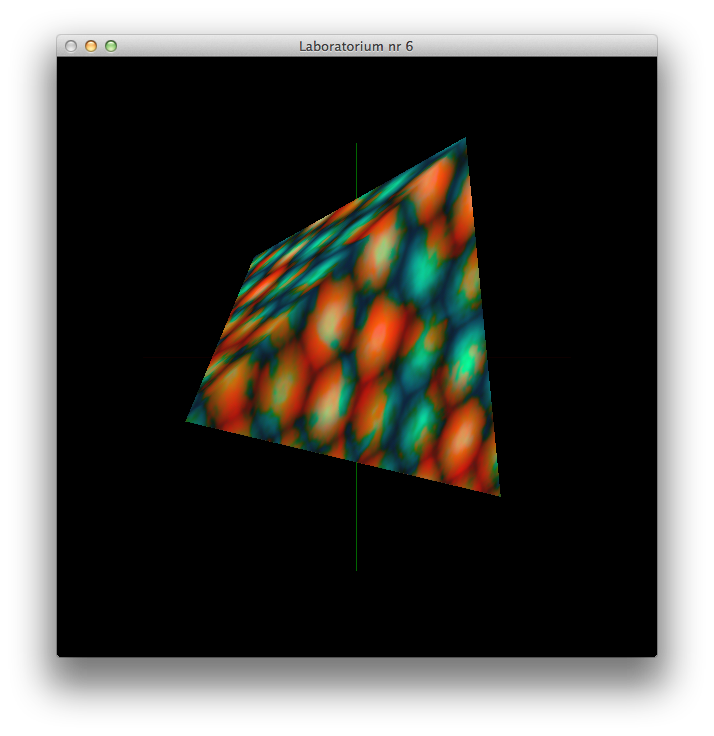
\includegraphics[width=\textwidth]{1.png}
      \caption{Oteksturowana piramida}
    \end{center}
  \end{figure}

  \begin{figure}[h!]
    \begin{center}
      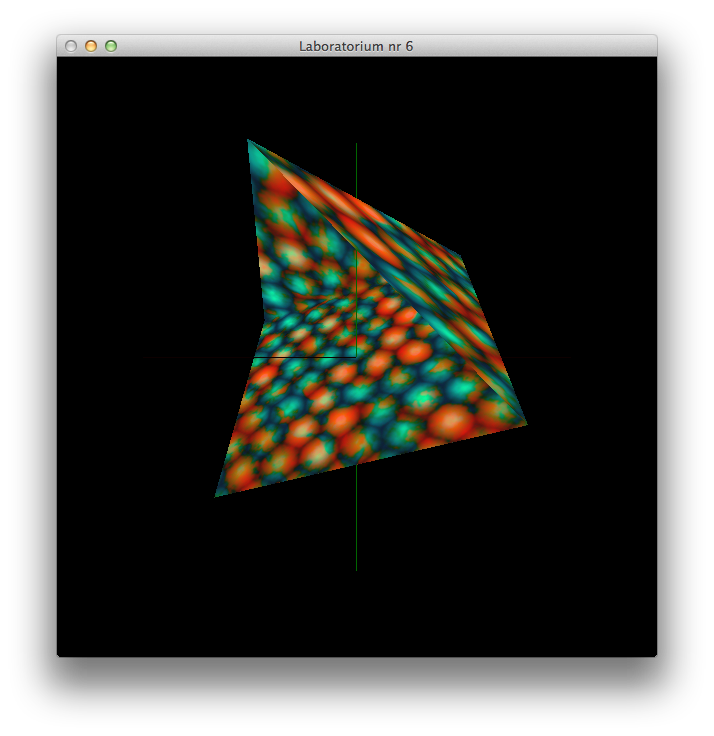
\includegraphics[width=\textwidth]{2.png}
      \caption{Oteksturowana piramida z widocznymi trzema ścianami}
    \end{center}
  \end{figure}

  \paragraph{}
  Warto przy okazji zwrócic uwage na parametr \texttt{GL\_CULL\_FACE}, który odpowiada za teksturowanie obu stron lub tylko jednej wieloboku. Ustawienie tego parametru poprzez wywołanie funkcji \texttt{glEnable(GL\_CULL\_FACE)} pozwala na uniknięcie obliczeń teksturowania wewnętrznych ścian obiektów.\texttt{}


  \newpage

  \section{Teksturowane jajko}
  \paragraph{}
  Kolejnym zadaniem było narysowanie jajka z poprzednich zajęc tym razem z wykorzystaniem tekstury. W tym celu należało zamienić wywołania funkcji \texttt{glColor3v} na \texttt{glTexCoord2f} z odpowiednimi parametrami.

  \paragraph{}
  \lstinputlisting{3.cpp}


  \begin{figure}[h!]
    \begin{center}
      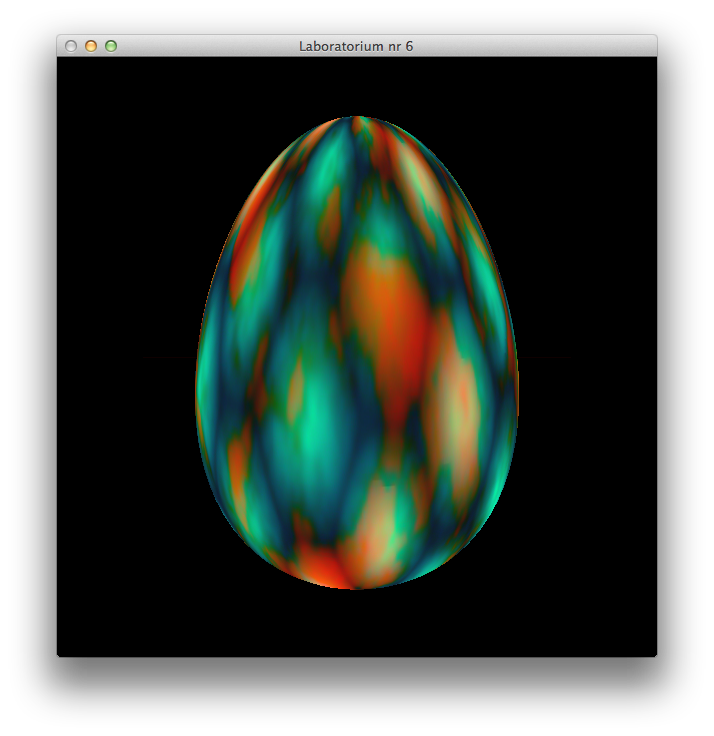
\includegraphics[width=\textwidth]{3.png}
      \caption{Oteksturowane jajko}
    \end{center}
  \end{figure}

  \newpage

  \section{Wnioski}
  \paragraph{}
  Teksturowanie obiektów 3-D z użyciem biblioteki OpenGL nie jest skomplikowanym zadaniem. Należy jednak pamiętać o odpowiednim przeliczaniu parametrów punktów tekstury. Problemem okazało się też samo wczytywanie tekstury wynikające z różnic implmentacji pod systemami Windows oraz Max OS X.
\end{document}